\documentclass[a4paper, fontsize=14pt]{article}
\usepackage[T2A]{fontenc}
\usepackage{mathtools}
\usepackage[utf8]{inputenc}
\usepackage[english, russian]{babel}
\usepackage{fancyhdr}
\usepackage{graphicx}
\usepackage{gensymb}
\usepackage{floatrow}
\usepackage{titlesec}
\usepackage{lastpage}
\usepackage{float}
\usepackage{gensymb}
\usepackage{booktabs}
\usepackage{amsmath}
\usepackage{amssymb}


\pagestyle{fancy}
	\fancyhf{}
	\lhead{\hspace{1bp} Работа \textnumero 3.5.3}
	\rhead{Терехов Максим 876\hspace{1bp}}
	\lfoot{Релаксационные колебания}
	\cfoot{\textbf{}}
	\rfoot{\thepage\ \textnormal{из}\ \pageref{LastPage}}
	\renewcommand{\headrulewidth}{1pt}
	\renewcommand{\footrulewidth}{1pt}


%\addtolength{\hoffset}{-1.75cm}
%\addtolength{\textwidth}{3.5cm} 

%\addtolength{\voffset}{-1.5cm}
%\addtolength{\textheight}{3cm} 

\titleformat{\section}
    [block]{\normalfont\bfseries\large}{\rlap{\thesection}}{0em}
    {\vspace{-0.02\textwidth}\begin{minipage}[t]{.95\textwidth}}
[\end{minipage}]

\thispagestyle{fancy}

\begin{document}
\selectlanguage{russian}


\huge
\centering
\textbf{Релаксационные колебания}

\raggedright
\parindent=1cm
\large
\section*{Цель работы}
	Изучение вольт-амперной характеристики нормального тлеющего разряда; исследование релаксационного генератора на стабилитроне.
\section*{Оборудование}
	Стабилитрон СГ-2 (газонаполненный диод) на монтажной панели, амперметр, вольтметр, магазин сопротивлений, магазин ёмкостей, источник питания, осциллограф (ЭО), генератор звуковой частоты (ЗГ).
\section*{Экспериментальная установка}
	\begin{figure}[H]
		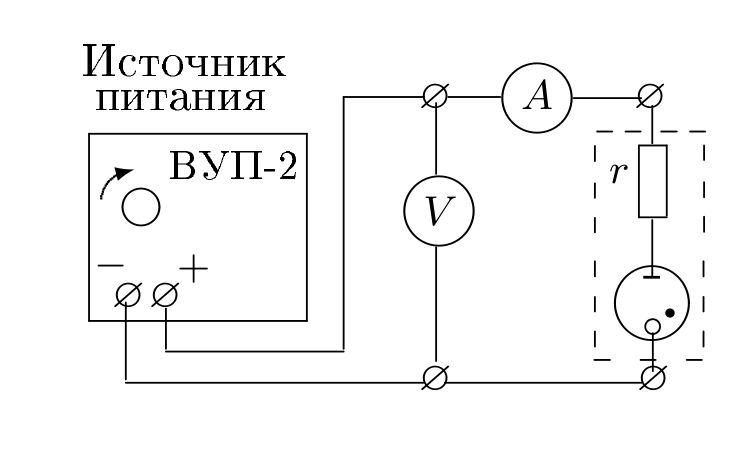
\includegraphics[width = 1.0\linewidth]{ust1.png}
		\caption{Схема установки для изучения характеристик стабилитрона}
	\end{figure}
	\begin{figure}[H]
		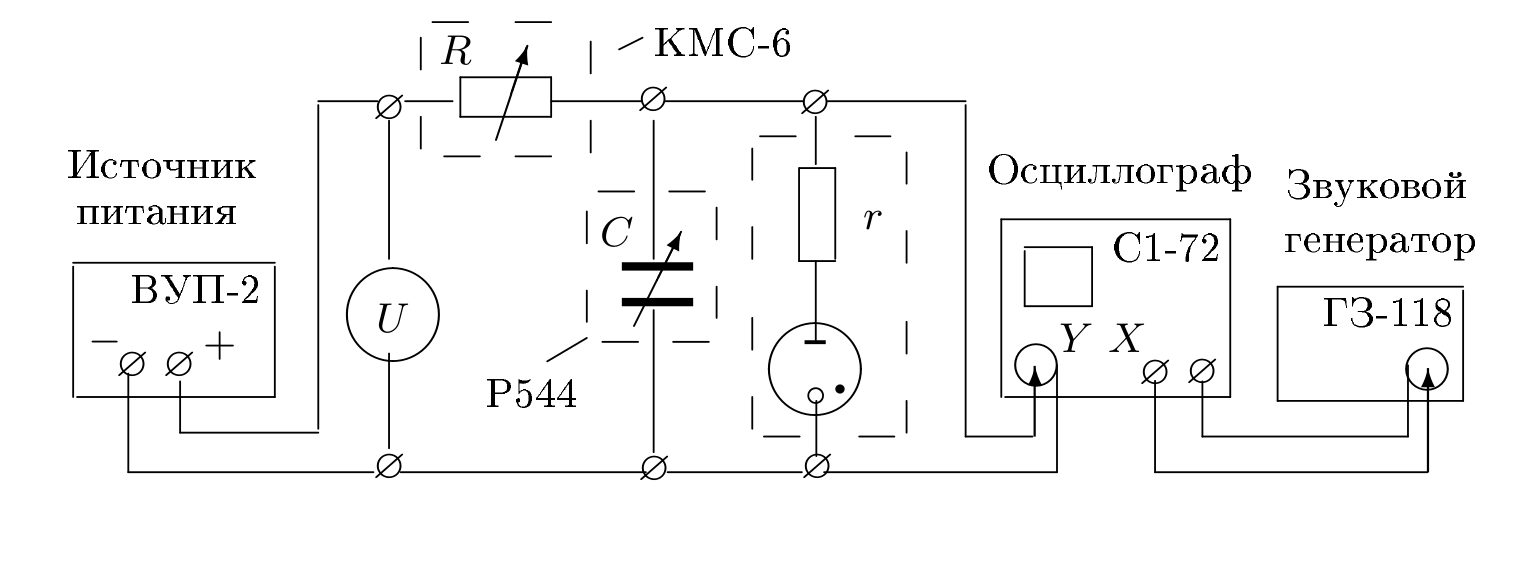
\includegraphics[width = 1.0\linewidth]{ust2.png}
		\caption{Схема установки для исследования релаксационных колебаний}
	\end{figure}
\section*{Теоретическая часть}
Колебательные системы, как правило, имеют два накопителя энергии, между которыми происходит её перекачка. В контуре, содержащем конденсатор и катушку индуктивности, электрическая энергия переходит в магнитную и обратно.

Встречается, однако, колебательные системы, содержащие всего один накопитель энергии. Рассмотрим в качестве примера электрическую цепь, содержащую конденсатор и сопротивление без самоиндукции. Разряд конденсатора через сопротивление представляет собой апериодический процесс. Разряду, однако, можно придать периодический характер, возобновляя заряд конденсатора через постоянные промежутки времени. Колебания в этом случае являются совокупностью двух апериодических процессов --- процесса зарядки конденсатора и процесса его разрядки.

\begin{figure}[H]
		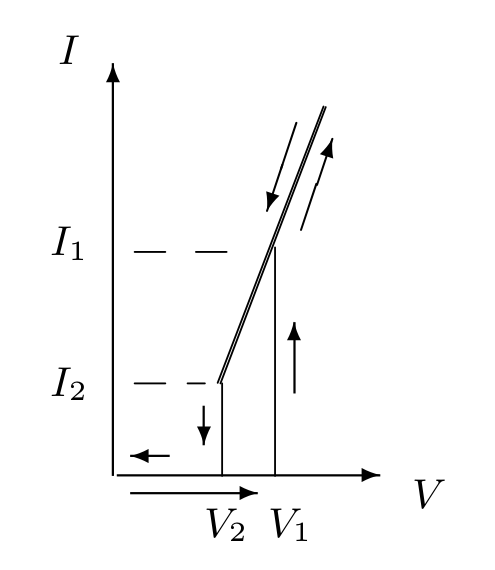
\includegraphics[width = 0.3\linewidth]{va.png}
		\caption{Вольт-амперная характеристика стабилитрона с поледовательно включённым резистором}
	\end{figure}
В нашей установке роль <<ключа>>, обеспечивающего попеременную зарядку и разрядку конденсатора, играет газоразрядный диод. Зависимость тока от напряжения для газоразрядной лампы не подчиняется закону Ома и характеризуется рядом особенностей. При малых напряжениях лампа практически не пропускает тока. Ток в лампе возникает только в том случае, если разность потенциалов на её электродах достигает напряжения зажигания $V_1 = V_\text{заж}$. При этом скачком устанавливается конечная сила тока $I_1$ --- в лампе возникает нормальный тлеющий разряд. При дальнейшем незначительном увеличении напряжения сила тока заметно возрастает по закону, близкому к линейному. Нормальный тлеющий разряд --- стабилизатор напряжения, отсюда второе название лампы --- стабиловольт.

Если начать уменьшать напряжение на горящей лампе, то при напряжении, равном $V_\text{заж}$, лампа ещё не гаснет, а сила тока продолжает уменьшаться. Лампа перестаёт пропускать ток лишь при напряжении гашения $V_2 = V_\text{гаш}$, которое обычно существенно меньше $V_\text{заж}$. Сила тока при этом скачком падает от значения $I_2 (I_2 < I_1)$ до нуля.

Изображённая выше вольт-амперная характеристика несколько идеализированна. У реальной лампы зависимость $I(V)$ не вполне линейна. При $V > V_\text{заж}$ графики, соответствующие возрастанию и убыванию напряжения, не всегда совпадают. Эти отличия, впрочем, носят второстепенный характер и для нашей задачи несущественны.

\begin{figure}[H]
		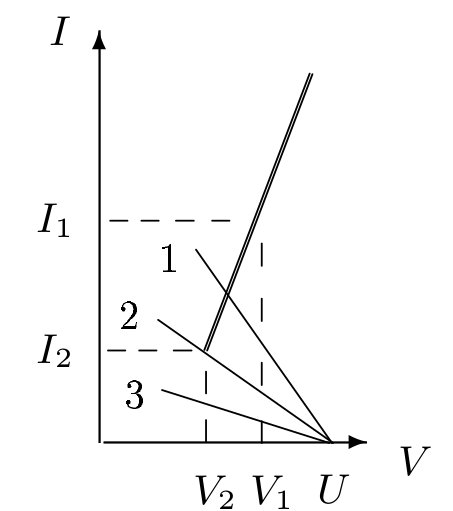
\includegraphics[width = 0.3\linewidth]{r.png}
		\caption{Режимы работы релаксационного генератора}
	\end{figure}
	Рассмотрим схему релаксационного генератора. Пусть напряжение батареи $U$ больше напряжения зажигания $V_1$. В обозначениях, принятых на схеме, справедливо уравнение
	\[
		I_C + I(V) = \frac{U - V}{R},
	\]
	или 
	\[
		C \frac{dV}{dt} + I(V) = \frac{U - V}{R}.
	\]
	В стационарном режиме работы, когда напряжение $V$ yа конденсаторе постоянно и $dV / dt = 0$, ток через лампу равен
	\[
		I_\text{ст} = \frac{U - V}{R}.
	\]
Это равенство представлено выше графически.

При разных $R$ графики имеют вид прямых, пересекающихся в точке $V = U, I = 0$. Область, где эти нагрузочные прямые пересекают вольт-амперную характеристику лампы, соответствует стационарному режиму --- при малых $R$ (прямая 1) лампа горит постоянно, колебания отсутствуют. Прямая 2, проходящая через точку $(I_2, V_2)$, соответствует критическому сопротивлению 
\[
	R_\text{кр} = \frac{U - V_2}{I_2}.
\]
При сопротивлении $R > R_\text{кр}$ нагрузочная прямая 3 не пересекает характеристику лампы, поэтому стационарный режим невозможен. В этом случае в системе устанавливаются колебания.

Рассмотрим, как происходит колебательный процесс. Пусть  вначале опыта ключ $K$ разомкнут и $V = 0$. Замкнём ключ. Конденсатор $C$ начинает заряжаться через сопротивление $R$, напряжение на нём увеличивается. Как только оно достигнет напряжения зажигания $V_\text{заж}$, лампа начинает проводить ток, причём прохождение тока сопровождается разрядкой конденсатора. В самом деле, батарея $U$, подключённая через большое сопротивление $R$, не может поддерживать необходимую для горения лампы величину тока. Во время горения лампы конденсатор разряжается, и когда напряжение на нём достигнет потенциала гашения, лампа перестанет проводить ток, а конденсатор вновь начнёт заряжаться. Возникают релаксационные колебания с амплитудой, равной $(V_1 - V_2)$.

\begin{figure}[H]
		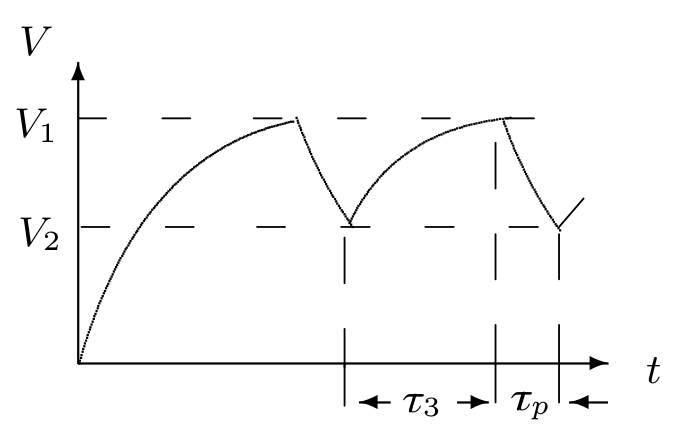
\includegraphics[width = 0.4\linewidth]{kol.png}
		\caption{Осциллограмма релаксационных колебаний}
	\end{figure}
Рассчитаем период колебаний. Полное время одного периода колебаний $T$ состоит из суммы времени зарядки $\tau_\text{з}$ и времени разрядки $\tau_\text{р}$, но если сопротивление $R$ существенно превосходит сопротивление зажжённой лампы, то $\tau_\text{з} \gg \tau_\text{р}$ и $T \approx \tau_\text{з}$. Во время зарядки конденсатора лампа не горит $(I(V) = 0)$, и уравнение приобретает вид
\[
	RC \frac{dV}{dt} = U - V.
\]
Будем отсчитывать время с момента гашения лампы, так что $V = V_2$ при $t = 0$. Решив это уравнение, найдём
\[
	V = U - (U - V_2) e^{-t / RC}.
\]
В момент зажигания $t = \tau_\text{з}, V = V_1$, поэтому
\[
	V_1 = U - (U - V_2) e^{\tau_\text{з} / RC}.
\]
Из этих двух уравнений нетрудно найти период колебаний:
\[
	T \approx \tau_\text{з} = RC \ln \frac{U - V_2}{U - V_1}.
\]
\section*{Обработка результатов измерений}
Исследуем вольт-амперную характеристику стабилитрона и построим график режима работы релаксационного генератора ($I = f(V)$):
\[
r = 5.1\ \text{кОм}
\]
\begin{figure}[H]
		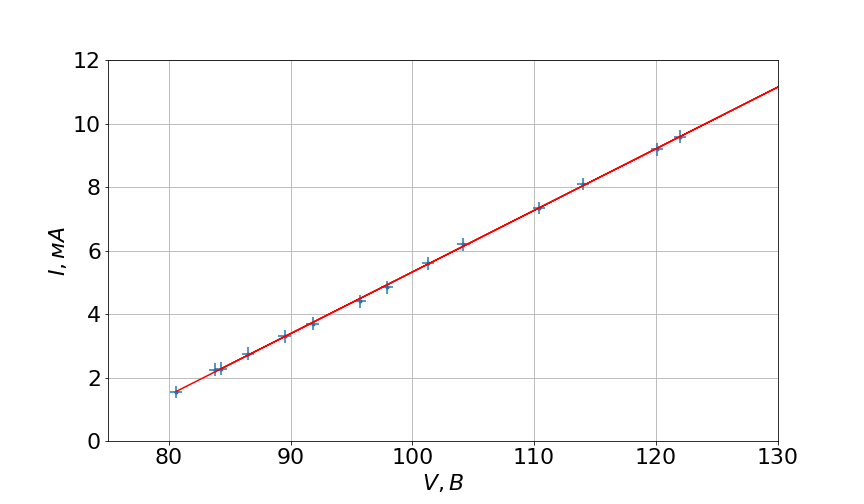
\includegraphics[width = 1.0\linewidth]{1.png}
		\caption{График зависимости $I$ от $V$}
	\end{figure}
	\[
		V_\text{заж} = 84.3\ B; \quad V_\text{гаш} = 80.2\ B
	\]
	\[
		R_\text{кр} = 19 \cdot 10^4\ \text{Ом}
	\]
	\begin{figure}[H]
		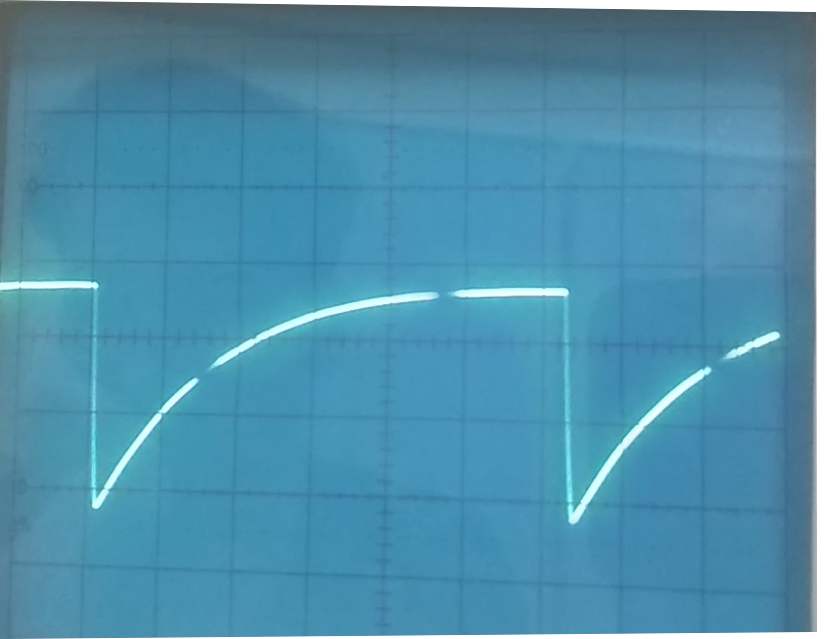
\includegraphics[width = 0.8\linewidth]{pila.png}
		\caption{Осциллограмма релаксационных колебаний}
	\end{figure}
Рассчитаем экспериментальные и теоретические значения периодов, построим графики зависимости $T_\text{эксп}$ и $T_\text{теор}:$
\[
	T \approx RC \ln \frac{U - V_\text{гаш}}{U - V_\text{заж}}
\]
\begin{figure}[H]
		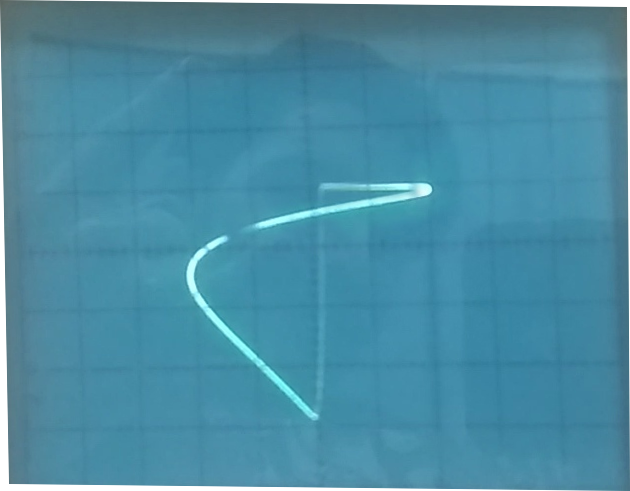
\includegraphics[width = 0.8\linewidth]{liss1.png}
		\caption{Фигура Лиссажу при отношении частот 1:1}
	\end{figure}
	\begin{figure}[H]
		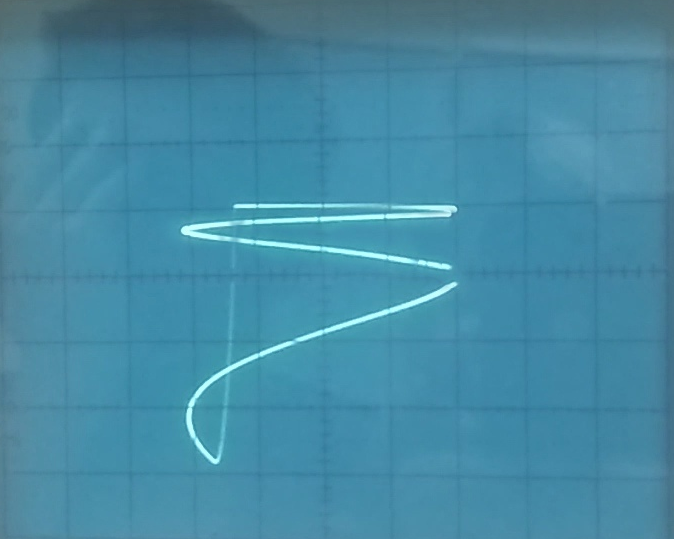
\includegraphics[width = 0.8\linewidth]{liss2.png}
		\caption{Фигура Лиссажу при отношении частот 2:1}
	\end{figure}
	\begin{figure}[H]
		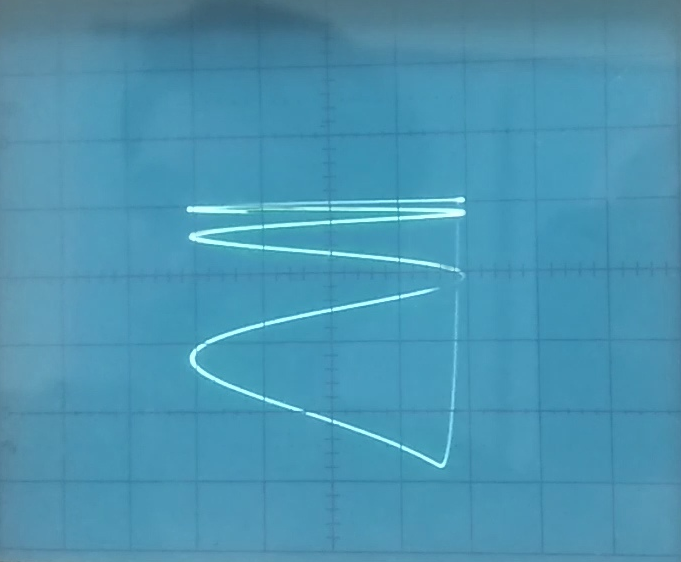
\includegraphics[width = 0.8\linewidth]{liss3.png}
		\caption{Фигура Лиссажу при отношении частот 3:1}
	\end{figure}
\begin{figure}[H]
		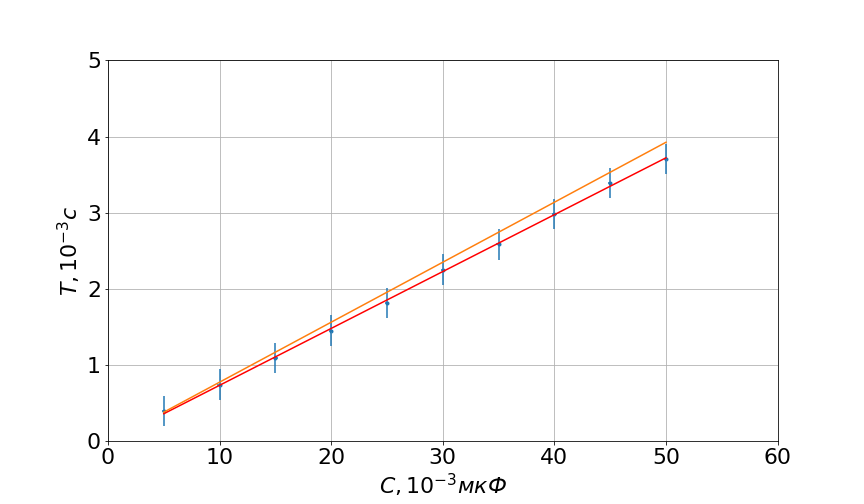
\includegraphics[width = 1.0\linewidth]{2.png}
		\caption{$T = f(C)$}
	\end{figure}
	\begin{figure}[H]
		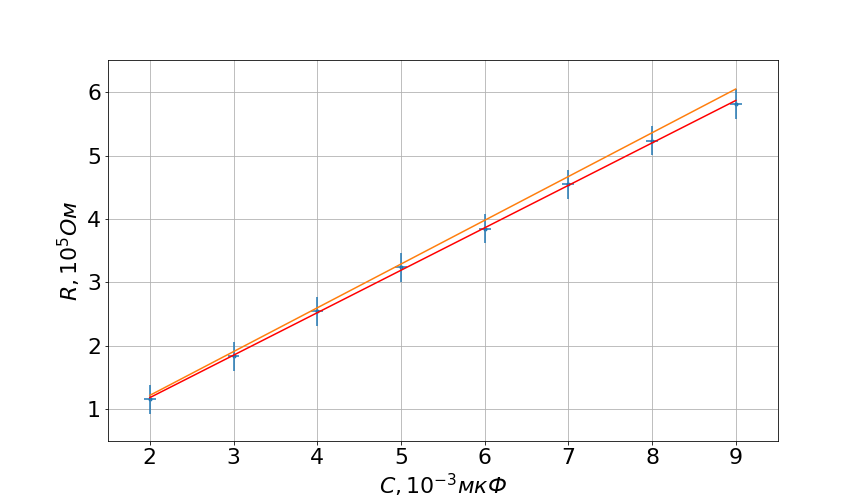
\includegraphics[width = 1.0\linewidth]{3.png}
		\caption{$T = f(R)$}
	\end{figure}
\section*{Вывод}
Мы исследовали волльт-амперную характеристику стабилитрона и убедились в том, что стабилитрон не подчиняется закону Ома и характеризуется рядом особенностей. При малых напряжениях лампа не пропускает ток вовсе, а при достижении напряжения зажигания --- в лампе возникает нормальный тлеющий разряд, который при незначительном увеличении напряжения сила тока линейно возрастает. При напряжении, незначительно меньшем, чем напряжение гашения, то возникают релаксационные колебания.

\end{document}